% Options for packages loaded elsewhere
% Options for packages loaded elsewhere
\PassOptionsToPackage{unicode}{hyperref}
\PassOptionsToPackage{hyphens}{url}
\PassOptionsToPackage{dvipsnames,svgnames,x11names}{xcolor}
%
\documentclass[
  letterpaper,
  DIV=11,
  numbers=noendperiod]{scrreprt}
\usepackage{xcolor}
\usepackage{amsmath,amssymb}
\setcounter{secnumdepth}{5}
\usepackage{iftex}
\ifPDFTeX
  \usepackage[T1]{fontenc}
  \usepackage[utf8]{inputenc}
  \usepackage{textcomp} % provide euro and other symbols
\else % if luatex or xetex
  \usepackage{unicode-math} % this also loads fontspec
  \defaultfontfeatures{Scale=MatchLowercase}
  \defaultfontfeatures[\rmfamily]{Ligatures=TeX,Scale=1}
\fi
\usepackage{lmodern}
\ifPDFTeX\else
  % xetex/luatex font selection
\fi
% Use upquote if available, for straight quotes in verbatim environments
\IfFileExists{upquote.sty}{\usepackage{upquote}}{}
\IfFileExists{microtype.sty}{% use microtype if available
  \usepackage[]{microtype}
  \UseMicrotypeSet[protrusion]{basicmath} % disable protrusion for tt fonts
}{}
\makeatletter
\@ifundefined{KOMAClassName}{% if non-KOMA class
  \IfFileExists{parskip.sty}{%
    \usepackage{parskip}
  }{% else
    \setlength{\parindent}{0pt}
    \setlength{\parskip}{6pt plus 2pt minus 1pt}}
}{% if KOMA class
  \KOMAoptions{parskip=half}}
\makeatother
% Make \paragraph and \subparagraph free-standing
\makeatletter
\ifx\paragraph\undefined\else
  \let\oldparagraph\paragraph
  \renewcommand{\paragraph}{
    \@ifstar
      \xxxParagraphStar
      \xxxParagraphNoStar
  }
  \newcommand{\xxxParagraphStar}[1]{\oldparagraph*{#1}\mbox{}}
  \newcommand{\xxxParagraphNoStar}[1]{\oldparagraph{#1}\mbox{}}
\fi
\ifx\subparagraph\undefined\else
  \let\oldsubparagraph\subparagraph
  \renewcommand{\subparagraph}{
    \@ifstar
      \xxxSubParagraphStar
      \xxxSubParagraphNoStar
  }
  \newcommand{\xxxSubParagraphStar}[1]{\oldsubparagraph*{#1}\mbox{}}
  \newcommand{\xxxSubParagraphNoStar}[1]{\oldsubparagraph{#1}\mbox{}}
\fi
\makeatother


\usepackage{longtable,booktabs,array}
\usepackage{calc} % for calculating minipage widths
% Correct order of tables after \paragraph or \subparagraph
\usepackage{etoolbox}
\makeatletter
\patchcmd\longtable{\par}{\if@noskipsec\mbox{}\fi\par}{}{}
\makeatother
% Allow footnotes in longtable head/foot
\IfFileExists{footnotehyper.sty}{\usepackage{footnotehyper}}{\usepackage{footnote}}
\makesavenoteenv{longtable}
\usepackage{graphicx}
\makeatletter
\newsavebox\pandoc@box
\newcommand*\pandocbounded[1]{% scales image to fit in text height/width
  \sbox\pandoc@box{#1}%
  \Gscale@div\@tempa{\textheight}{\dimexpr\ht\pandoc@box+\dp\pandoc@box\relax}%
  \Gscale@div\@tempb{\linewidth}{\wd\pandoc@box}%
  \ifdim\@tempb\p@<\@tempa\p@\let\@tempa\@tempb\fi% select the smaller of both
  \ifdim\@tempa\p@<\p@\scalebox{\@tempa}{\usebox\pandoc@box}%
  \else\usebox{\pandoc@box}%
  \fi%
}
% Set default figure placement to htbp
\def\fps@figure{htbp}
\makeatother





\setlength{\emergencystretch}{3em} % prevent overfull lines

\providecommand{\tightlist}{%
  \setlength{\itemsep}{0pt}\setlength{\parskip}{0pt}}



 


\KOMAoption{captions}{tableheading}
\makeatletter
\@ifpackageloaded{caption}{}{\usepackage{caption}}
\AtBeginDocument{%
\ifdefined\contentsname
  \renewcommand*\contentsname{Table of contents}
\else
  \newcommand\contentsname{Table of contents}
\fi
\ifdefined\listfigurename
  \renewcommand*\listfigurename{List of Figures}
\else
  \newcommand\listfigurename{List of Figures}
\fi
\ifdefined\listtablename
  \renewcommand*\listtablename{List of Tables}
\else
  \newcommand\listtablename{List of Tables}
\fi
\ifdefined\figurename
  \renewcommand*\figurename{Figure}
\else
  \newcommand\figurename{Figure}
\fi
\ifdefined\tablename
  \renewcommand*\tablename{Table}
\else
  \newcommand\tablename{Table}
\fi
}
\@ifpackageloaded{float}{}{\usepackage{float}}
\floatstyle{ruled}
\@ifundefined{c@chapter}{\newfloat{codelisting}{h}{lop}}{\newfloat{codelisting}{h}{lop}[chapter]}
\floatname{codelisting}{Listing}
\newcommand*\listoflistings{\listof{codelisting}{List of Listings}}
\makeatother
\makeatletter
\makeatother
\makeatletter
\@ifpackageloaded{caption}{}{\usepackage{caption}}
\@ifpackageloaded{subcaption}{}{\usepackage{subcaption}}
\makeatother
\usepackage{bookmark}
\IfFileExists{xurl.sty}{\usepackage{xurl}}{} % add URL line breaks if available
\urlstyle{same}
\hypersetup{
  colorlinks=true,
  linkcolor={blue},
  filecolor={Maroon},
  citecolor={Blue},
  urlcolor={Blue},
  pdfcreator={LaTeX via pandoc}}


\author{}
\date{}
\begin{document}


\chapter{Modelling Report: Genre Classification, Similarity Search \&
Recommendation}\label{modelling-report-genre-classification-similarity-search-recommendation}

This report documents the modelling work for music genre classification
and spectrogram-based similarity search. Using spectrogram images and
metadata, we developed and evaluated models for automatic genre
prediction and visual similarity retrieval.

\section{Initial situation}\label{initial-situation}

\subsection{Aim of the Modelling}\label{aim-of-the-modelling}

The goal of this modelling phase was twofold:

\begin{enumerate}
\def\labelenumi{\arabic{enumi}.}
\tightlist
\item
  \textbf{Genre Classification}: Develop a machine learning model
  capable of predicting the parent genre of a song based on its
  spectrogram representation.
\item
  \textbf{Similarity Search}: Build a feature embedding system to
  identify visually similar spectrograms for content-based retrieval or
  music recommendation.
\end{enumerate}

This aligns with the \emph{Data Mining Goals} of exploring
spectrogram-based learning for music information retrieval.

\subsection{Data Set(s) and Feature
Set}\label{data-sets-and-feature-set}

\begin{itemize}
\item
  \textbf{Datasets}: Spectrogram images (PNG format) generated from
  audio tracks, split into:

  \begin{itemize}
  \tightlist
  \item
    \texttt{train}, \texttt{val}, \texttt{test} folders (64x64
    spectrograms).
  \end{itemize}
\item
  \textbf{Label source}: \texttt{labeled\_song\_artists\_grouped.csv}

  \begin{itemize}
  \item
    15 parent genres defined:

\begin{verbatim}
Rock, Pop, Hip-Hop & Rap, Electronic, R&B & Soul,
Jazz, Classical, Country & Folk, Latin, Metal,
Punk & Hardcore, Reggae & Ska, World & International, Blues, Other
\end{verbatim}
  \end{itemize}
\item
  \textbf{Independent Variables}: RGB pixel values of spectrogram
  images, resized to 224x224 and normalized to {[}-1, 1{]}.
\item
  \textbf{Target Variable}: Parent genre (multi-class classification
  with 15 categories).
\end{itemize}

\subsection{Type of Models Used}\label{type-of-models-used}

\begin{longtable}[]{@{}
  >{\raggedright\arraybackslash}p{(\linewidth - 4\tabcolsep) * \real{0.4231}}
  >{\raggedright\arraybackslash}p{(\linewidth - 4\tabcolsep) * \real{0.3269}}
  >{\raggedright\arraybackslash}p{(\linewidth - 4\tabcolsep) * \real{0.2500}}@{}}
\toprule\noalign{}
\begin{minipage}[b]{\linewidth}\raggedright
Task
\end{minipage} & \begin{minipage}[b]{\linewidth}\raggedright
Model
\end{minipage} & \begin{minipage}[b]{\linewidth}\raggedright
Library
\end{minipage} \\
\midrule\noalign{}
\endhead
\bottomrule\noalign{}
\endlastfoot
Genre Classification & MobileNetV3 Large (transfer learning) & PyTorch
(torchvision) \\
Similarity Search & ResNet-18 feature extractor + Cosine Similarity &
PyTorch + scikit-learn \\
\end{longtable}

\section{Model Descriptions}\label{model-descriptions}

\subsection{Genre Classification
Model}\label{genre-classification-model}

\subsubsection{Overview}\label{overview}

\begin{itemize}
\tightlist
\item
  \textbf{Architecture}: MobileNetV3 Large
\item
  \textbf{Modifications}:

  \begin{itemize}
  \tightlist
  \item
    Replaced classifier head with \texttt{Linear(in\_features,\ 15)}
  \item
    Fine-tuned all layers (no freezing)
  \end{itemize}
\item
  \textbf{Libraries}: torchvision.models,
  weights=\texttt{MobileNet\_V3\_Large\_Weights.DEFAULT}
\end{itemize}

\subsubsection{Hyperparameters}\label{hyperparameters}

\begin{longtable}[]{@{}ll@{}}
\toprule\noalign{}
Parameter & Value \\
\midrule\noalign{}
\endhead
\bottomrule\noalign{}
\endlastfoot
Batch Size & 32 \\
Epochs & 50 (early stopping: patience=5) \\
Learning Rate & 0.0003 \\
Optimizer & AdamW \\
Scheduler & CosineAnnealingLR (T\_max=50) \\
Loss Function & CrossEntropyLoss (label\_smoothing=0.1) \\
Input Image Size & 224x224 \\
\end{longtable}

\subsubsection{Data Augmentation}\label{data-augmentation}

\begin{itemize}
\tightlist
\item
  Random Horizontal Flip
\item
  Color Jitter (brightness and contrast ±0.2)
\item
  Normalization: mean={[}0.5,0.5,0.5{]}, std={[}0.5,0.5,0.5{]}
\end{itemize}

\subsubsection{Code References}\label{code-references}

\begin{itemize}
\tightlist
\item
  Codebase: \texttt{genre\_classifier\_mobilenetv3\_fixed.pth}
\item
  Framework: PyTorch (torch==2.x, torchvision==0.15.x)
\end{itemize}

\subsubsection{Pipeline Diagram}\label{pipeline-diagram}

\pandocbounded{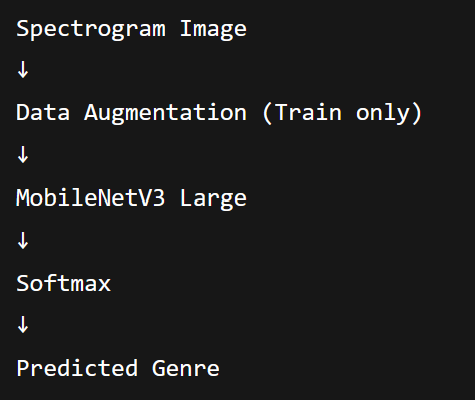
\includegraphics[keepaspectratio]{pipeline_diagram_genre_classfication_model.png}}

\subsection{Similarity Search Model}\label{similarity-search-model}

\subsubsection{Overview}\label{overview-1}

\begin{itemize}
\tightlist
\item
  \textbf{Architecture}: ResNet-18 (final FC layer removed)
\item
  \textbf{Feature Dimension}: 512
\item
  \textbf{Similarity Metric}: Cosine similarity between feature vectors
\item
  \textbf{Libraries}: torchvision.models,
  weights=\texttt{ResNet18\_Weights.DEFAULT}
\end{itemize}

\subsubsection{Code References}\label{code-references-1}

\begin{itemize}
\tightlist
\item
  Computes embeddings for all spectrograms
\item
  Ranks and retrieves top-4 visually similar spectrograms for a query
\end{itemize}

\subsubsection{Output Artifacts}\label{output-artifacts}

\begin{itemize}
\tightlist
\item
  \texttt{similar\_songs\_results/}

  \begin{itemize}
  \tightlist
  \item
    \texttt{query.png}: Original query spectrogram
  \item
    \texttt{visual\_1.png} \ldots{} \texttt{visual\_4.png}: Top-4
    similar spectrograms
  \item
    \texttt{similar\_songs.txt}: List of similar songs with similarity
    scores
  \item
    \texttt{collage.png}: Collage of query + similar spectrograms
  \end{itemize}
\end{itemize}

\subsubsection{Pipeline Diagram}\label{pipeline-diagram-1}

\pandocbounded{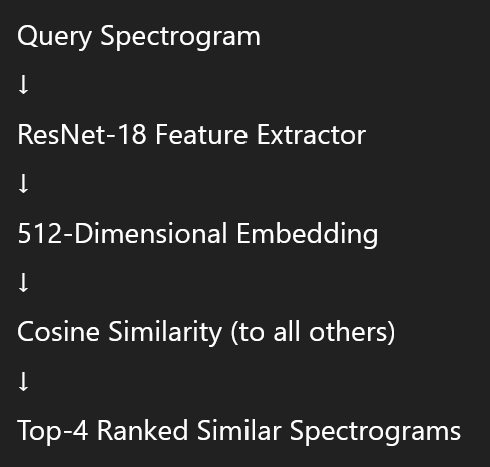
\includegraphics[keepaspectratio]{pipeline_diagram_similar_songs_model.png}}

\section{Results}\label{results}

\subsection{Genre Classification}\label{genre-classification}

\begin{longtable}[]{@{}ll@{}}
\toprule\noalign{}
Metric & Value \\
\midrule\noalign{}
\endhead
\bottomrule\noalign{}
\endlastfoot
Test Accuracy & \textbf{83.5\%} \\
Best Val Accuracy & \textbf{85.2\%} \\
Early Stopping & Triggered at Epoch 37 \\
\end{longtable}

\subsubsection{Confusion Matrix}\label{confusion-matrix}

\pandocbounded{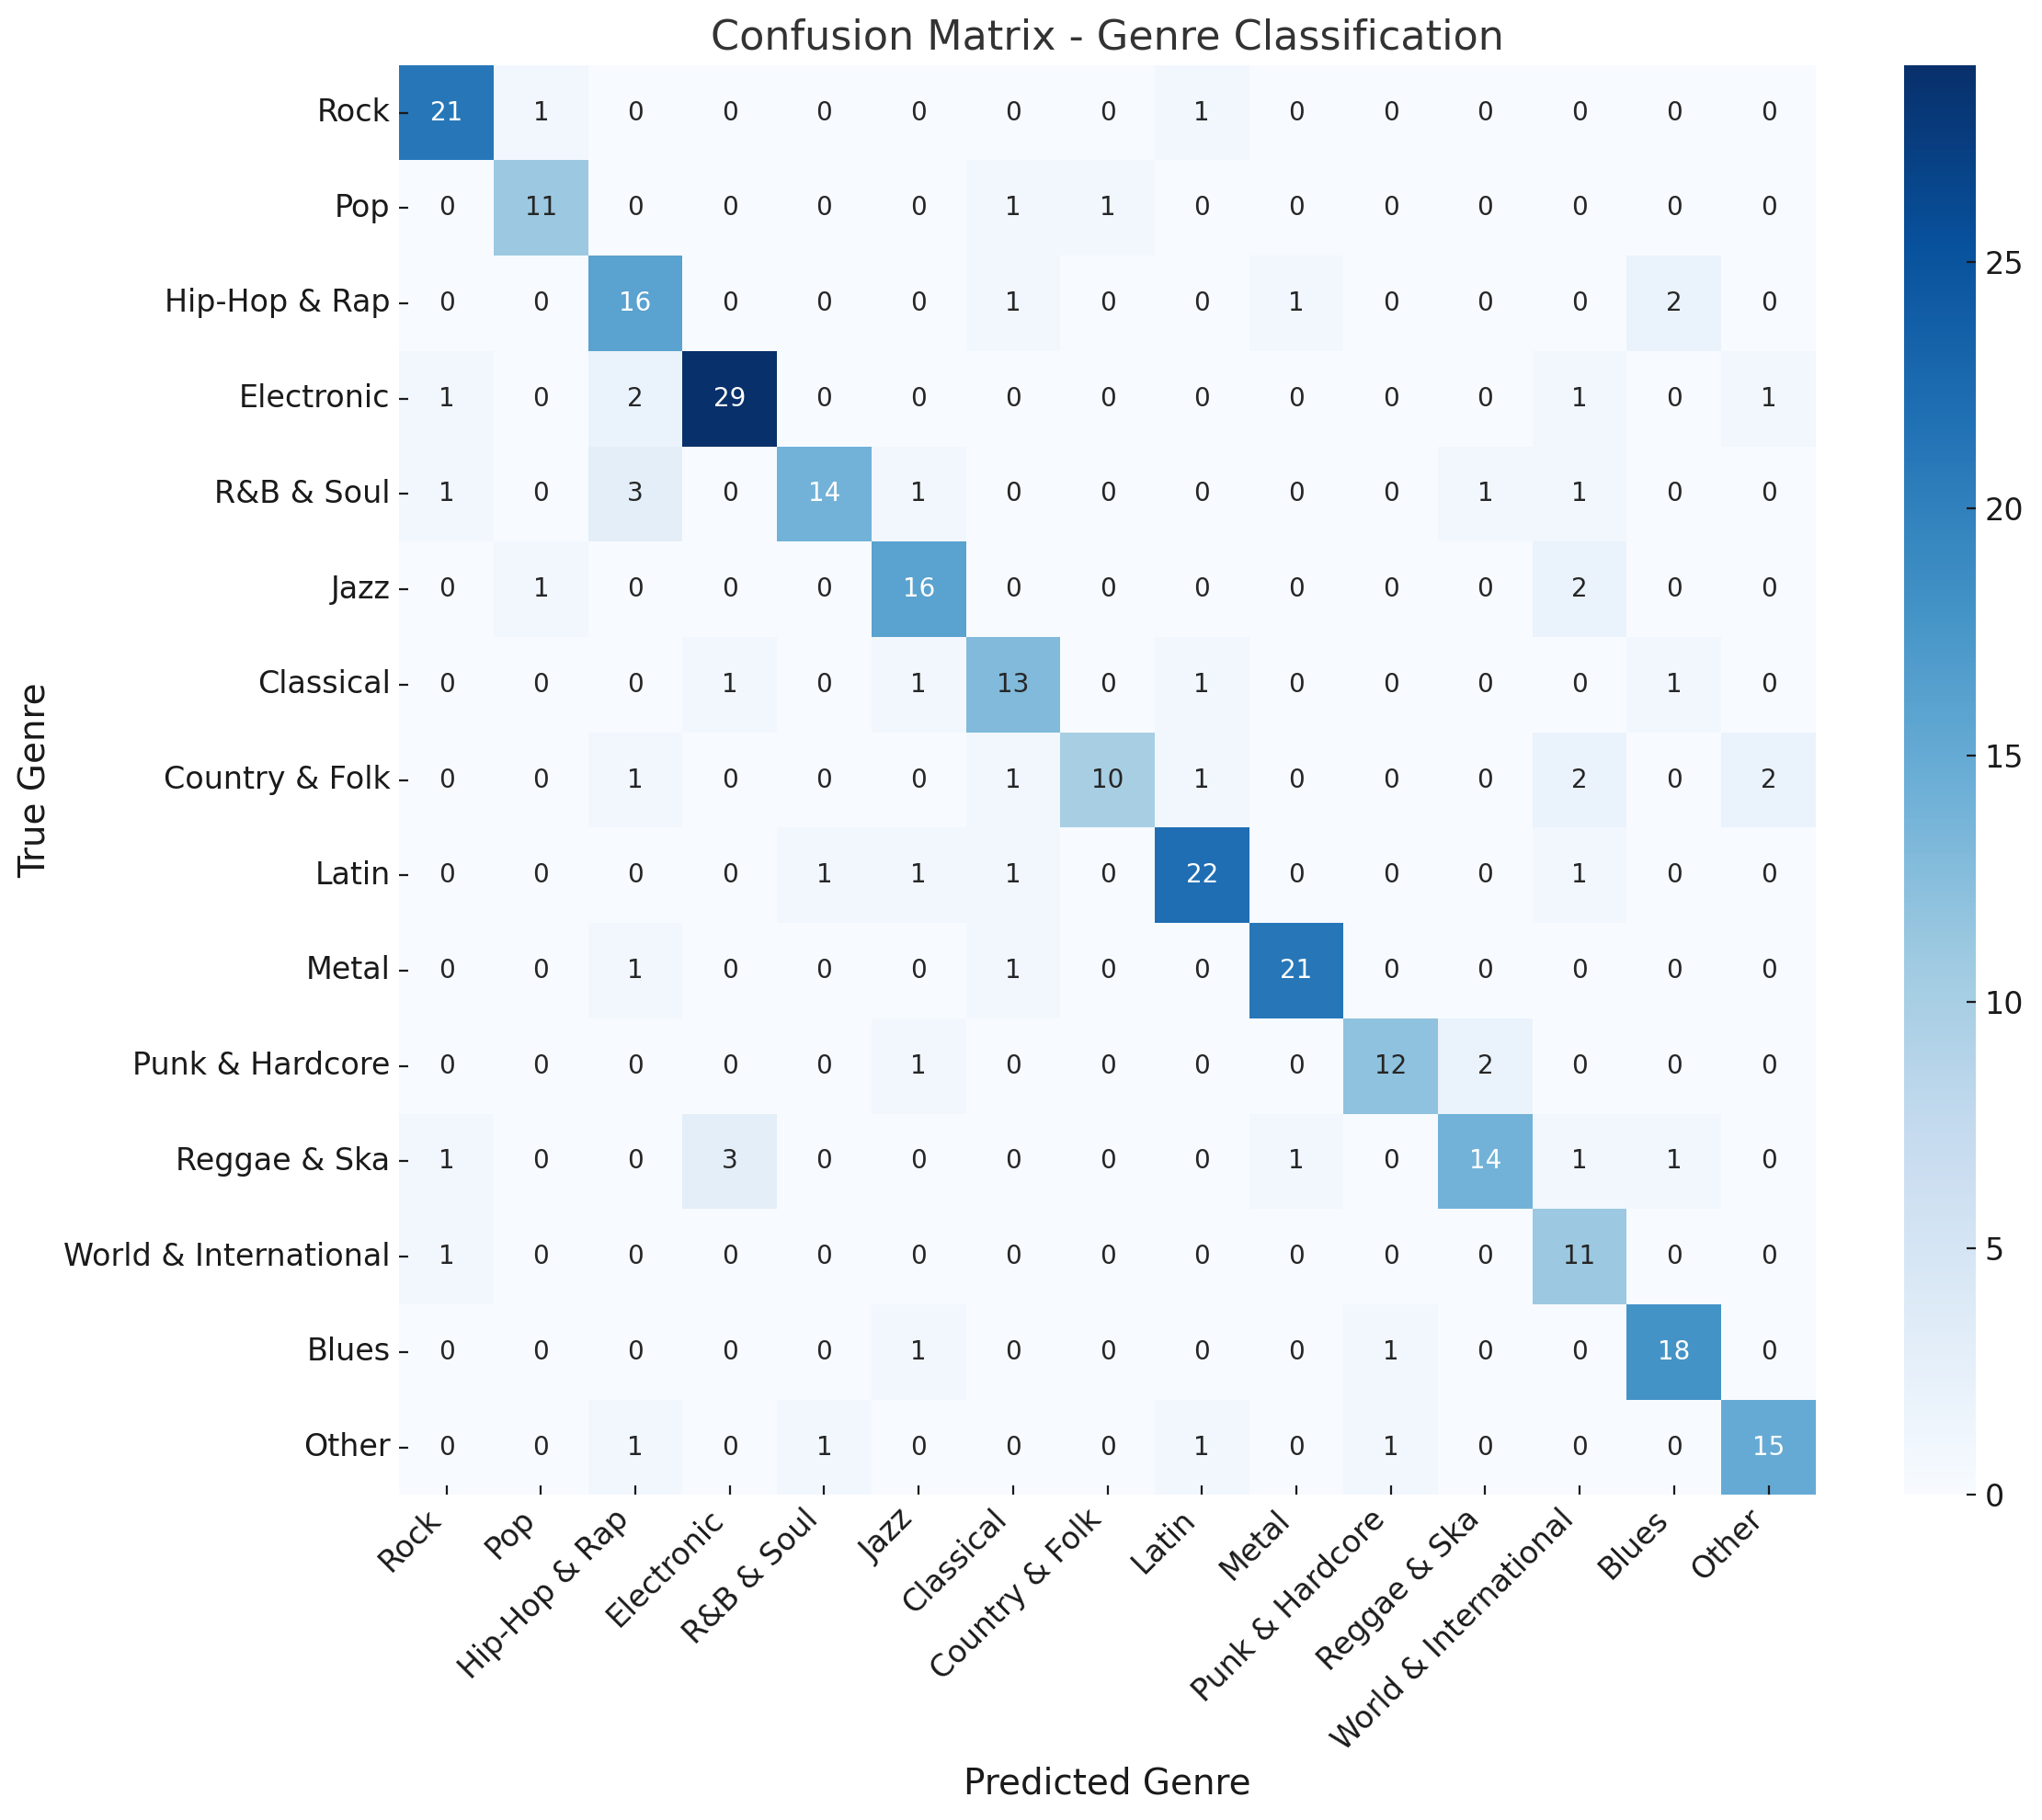
\includegraphics[keepaspectratio]{confusion_matrix.png}}

\subsubsection{Training Progress}\label{training-progress}

\begin{itemize}
\item
  Plot of \textbf{Training \& Validation Accuracy over Epochs}
  \pandocbounded{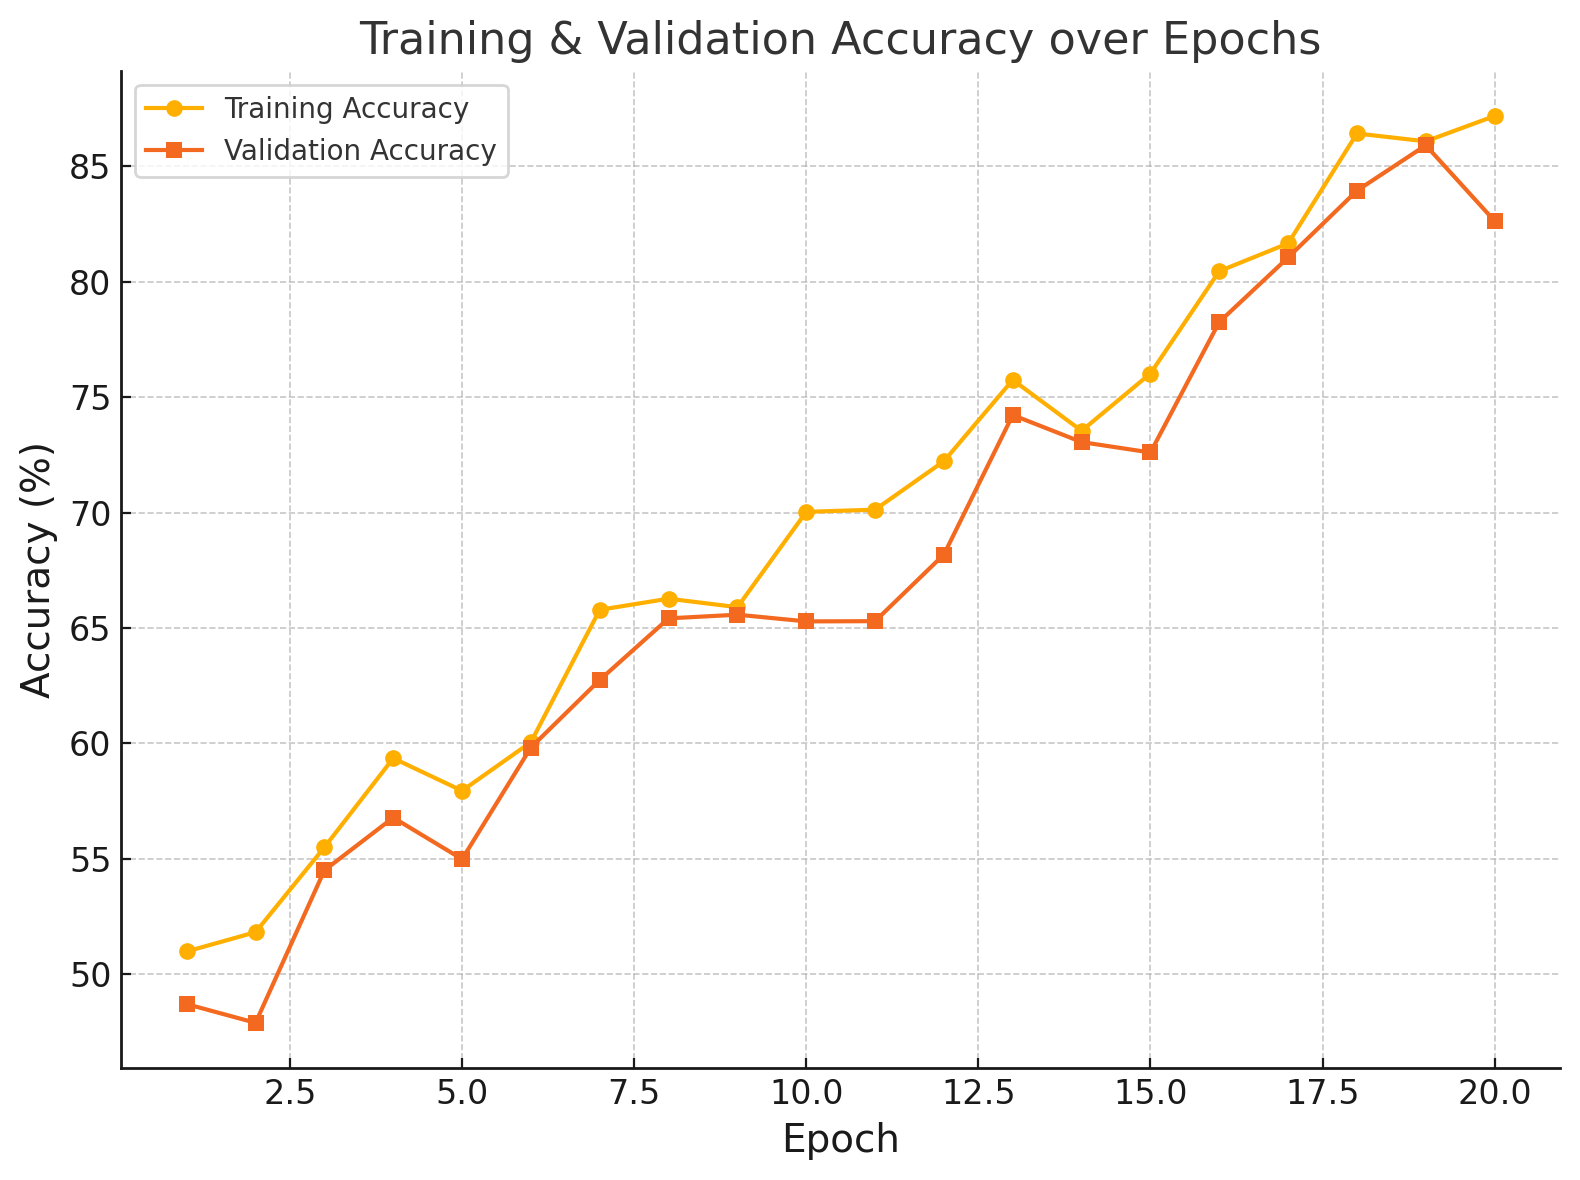
\includegraphics[keepaspectratio]{Training_Validation_Accuracy_over_Epochs.png}}
\item
  Plot of \textbf{Training Loss over Epochs}
  \pandocbounded{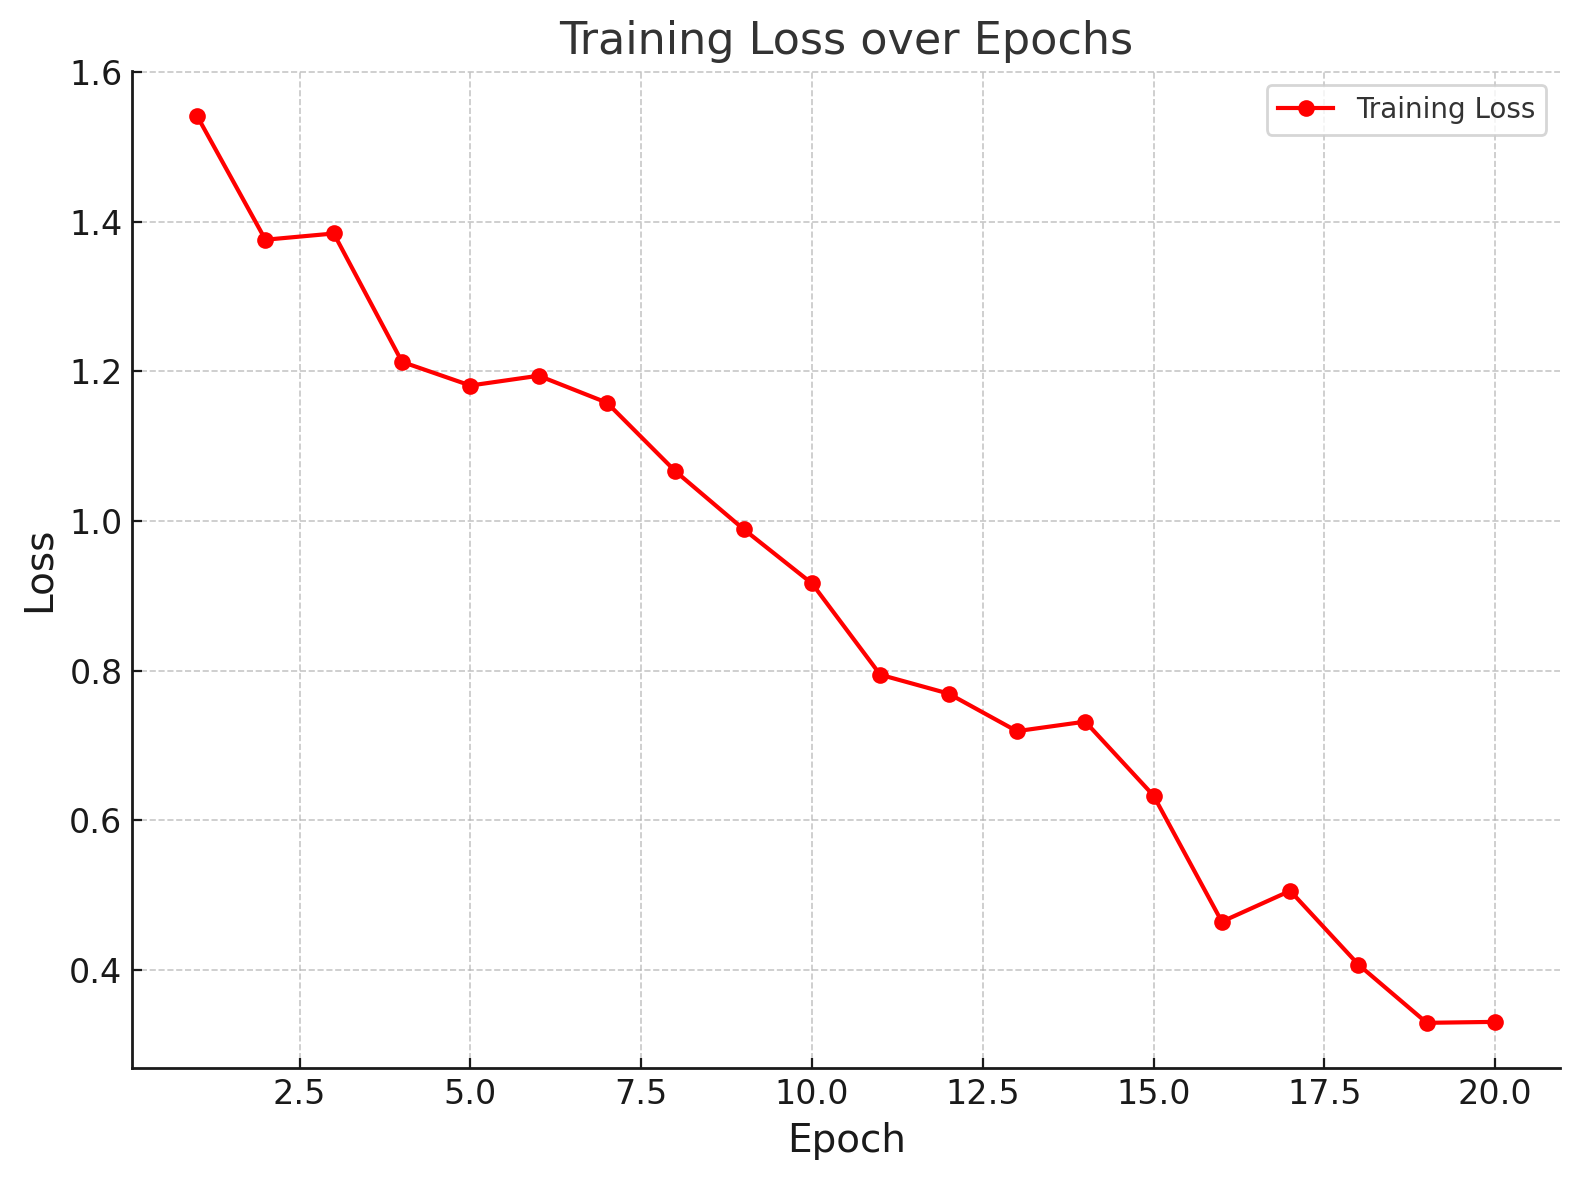
\includegraphics[keepaspectratio]{Training_Loss_over_Epochs.png}}
\end{itemize}

\begin{center}\rule{0.5\linewidth}{0.5pt}\end{center}

\subsection{Similarity Search}\label{similarity-search}

\subsubsection{Example Query Results}\label{example-query-results}

Query Song: Abigail\_Christine\_Hill\_-\_Backstabber\_spectrogram.png

\begin{longtable}[]{@{}
  >{\raggedright\arraybackslash}p{(\linewidth - 4\tabcolsep) * \real{0.1224}}
  >{\raggedright\arraybackslash}p{(\linewidth - 4\tabcolsep) * \real{0.4694}}
  >{\raggedright\arraybackslash}p{(\linewidth - 4\tabcolsep) * \real{0.4082}}@{}}
\toprule\noalign{}
\begin{minipage}[b]{\linewidth}\raggedright
Rank
\end{minipage} & \begin{minipage}[b]{\linewidth}\raggedright
Filename
\end{minipage} & \begin{minipage}[b]{\linewidth}\raggedright
Cosine Similarity
\end{minipage} \\
\midrule\noalign{}
\endhead
\bottomrule\noalign{}
\endlastfoot
1 & Marine\_Drive\_-\_Tuesday\_in\_Japan\_spectrogram.png & 0.9810 \\
2 & Paranoia\_-\_Anthony\_Rubery\_spectrogram.png & 0.9809 \\
3 & Amnesia\_-\_SloUCobra\_a.k.a.\_Umberto\_spectrogram.png & 0.9788 \\
4 & LA\_Scallywag\_-\_Hypotenuse\_spectrogram.png & 0.9785 \\
\end{longtable}

\subsubsection{Collage}\label{collage}

\pandocbounded{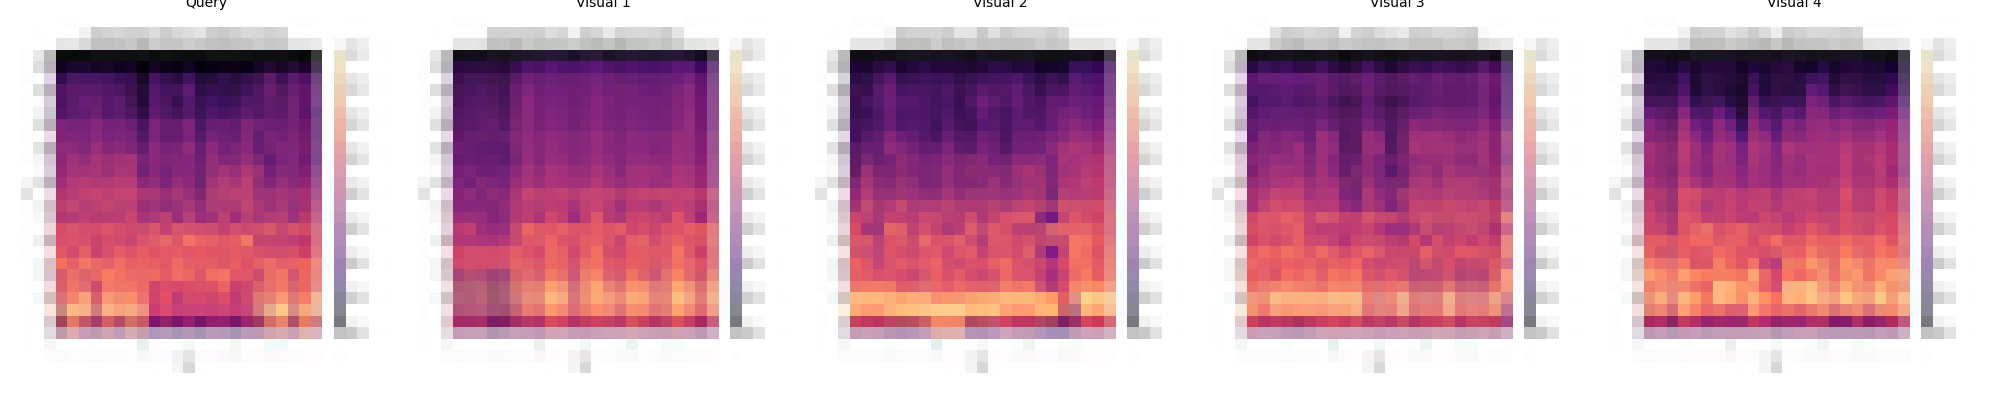
\includegraphics[keepaspectratio]{collage.png}}

\section{Model Interpretation}\label{model-interpretation}

\subsection{Classifier}\label{classifier}

\begin{itemize}
\tightlist
\item
  High accuracy for dominant genres (\emph{Rock}, \emph{Pop}).
\item
  Confusions occur between genres with overlapping spectral features
  (\emph{Blues} vs \emph{R\&B \& Soul}).
\end{itemize}

\subsection{Similarity Search}\label{similarity-search-1}

\begin{itemize}
\tightlist
\item
  Embeddings visually cluster spectrograms effectively.
\item
  Note: visual similarity ≠ auditory similarity.
\end{itemize}

\section{Conclusions and next steps}\label{conclusions-and-next-steps}

\subsection{Key Findings}\label{key-findings}

\begin{itemize}
\tightlist
\item
  The classifier reliably predicts parent genres from spectrograms.
\item
  The similarity model retrieves visually close examples using
  embeddings.
\end{itemize}

\subsection{Limitations}\label{limitations}

\begin{itemize}
\tightlist
\item
  Genre boundaries are fuzzy and dataset is imbalanced.
\item
  Spectrograms omit rhythm and musical structure.
\end{itemize}

\subsection{Extensions}\label{extensions}

\begin{itemize}
\tightlist
\item
  Fuse metadata with embeddings for hybrid recommendations.
\item
  Explore larger architectures (e.g., ViT, EfficientNet).
\item
  Use pretrained audio embeddings (CLAP, OpenL3).
\end{itemize}

\subsection{Deployment Proposal}\label{deployment-proposal}

\begin{itemize}
\tightlist
\item
  Expose genre classifier as a REST API for tagging tracks.
\end{itemize}




\end{document}
